% Build:  python fetch_benchmark_figs.py && pdflatex benchmarks.tex (twice)
\documentclass[11pt]{article}
\usepackage[margin=1in]{geometry}
\usepackage{amsmath,amssymb}
\usepackage{booktabs}
\usepackage{graphicx}
\usepackage{xcolor}
\usepackage{array}
\usepackage{enumitem}
\usepackage{float}
\usepackage[T1]{fontenc}
\usepackage[utf8]{inputenc}
\usepackage[colorlinks=true,linkcolor=black,citecolor=black,urlcolor=blue]{hyperref}

\definecolor{ink}{HTML}{1F2328}
\definecolor{sub}{HTML}{57606A}
\definecolor{panel}{HTML}{F6F8FA}
\definecolor{edge}{HTML}{D0D7DE}

\newcommand{\facts}[1]{\par\vspace{2pt}\noindent\colorbox{panel}{\parbox{\dimexpr\textwidth-2\fboxsep}{\small #1}}\vspace{4pt}}
\newcommand{\fit}[1]{\par\noindent\textbf{Fit for our study.} #1}
\setlist{itemsep=1pt, topsep=2pt}

\title{\textbf{Benchmarks for evaluation-driven program evolution}\\[2mm]
\large A survey for choosing the next test suite}
\author{Pantheon-Evolve}
\date{September 2026}

\begin{document}
\maketitle

\begin{abstract}
\noindent Our three-task study (AHC039, circle packing, Erd\H{o}s minimum overlap) taught one
lesson above the others: a benchmark that saturates cannot rank search methods. AHC039 turned
out to be bounded by its seed's ceiling, circle packing has a single attractor every method
finds, and Erd\H{o}s has a basin every method lands in. This document surveys twelve benchmarks
that an evaluation-driven code-evolution method (AlphaEvolve-style, SimpleTES-style, or our
LabNotebook) can be run on, gives a short introduction to each, states what it measures and what
it costs, and ends with a recommendation for the next suite.
\end{abstract}

\section{What we need from a benchmark}

A task is useful for \emph{comparing} search methods when it has, in order of importance:
\begin{enumerate}
  \item \textbf{Automatic, exact verification.} The score must come from a program, not a judge,
    and the same program must give the same score twice. Wall-clock scoring (AHC039, kernels)
    adds noise of the size of the effects being measured; we needed a dedicated serialized
    evaluation server to make it usable.
  \item \textbf{Headroom.} The best known result must be far enough from what a strong seed
    reaches that methods can separate. Two of our three tasks had none.
  \item \textbf{A continuous score.} Pass/fail collapses the signal; a speedup ratio or a bound
    keeps it.
  \item \textbf{Cheap evaluation.} A budget of 160--480 model calls should buy hundreds of
    measured candidates, not a handful.
  \item \textbf{Enough tasks} that one lucky problem cannot decide a comparison.
\end{enumerate}

\begin{figure}[H]
\centering
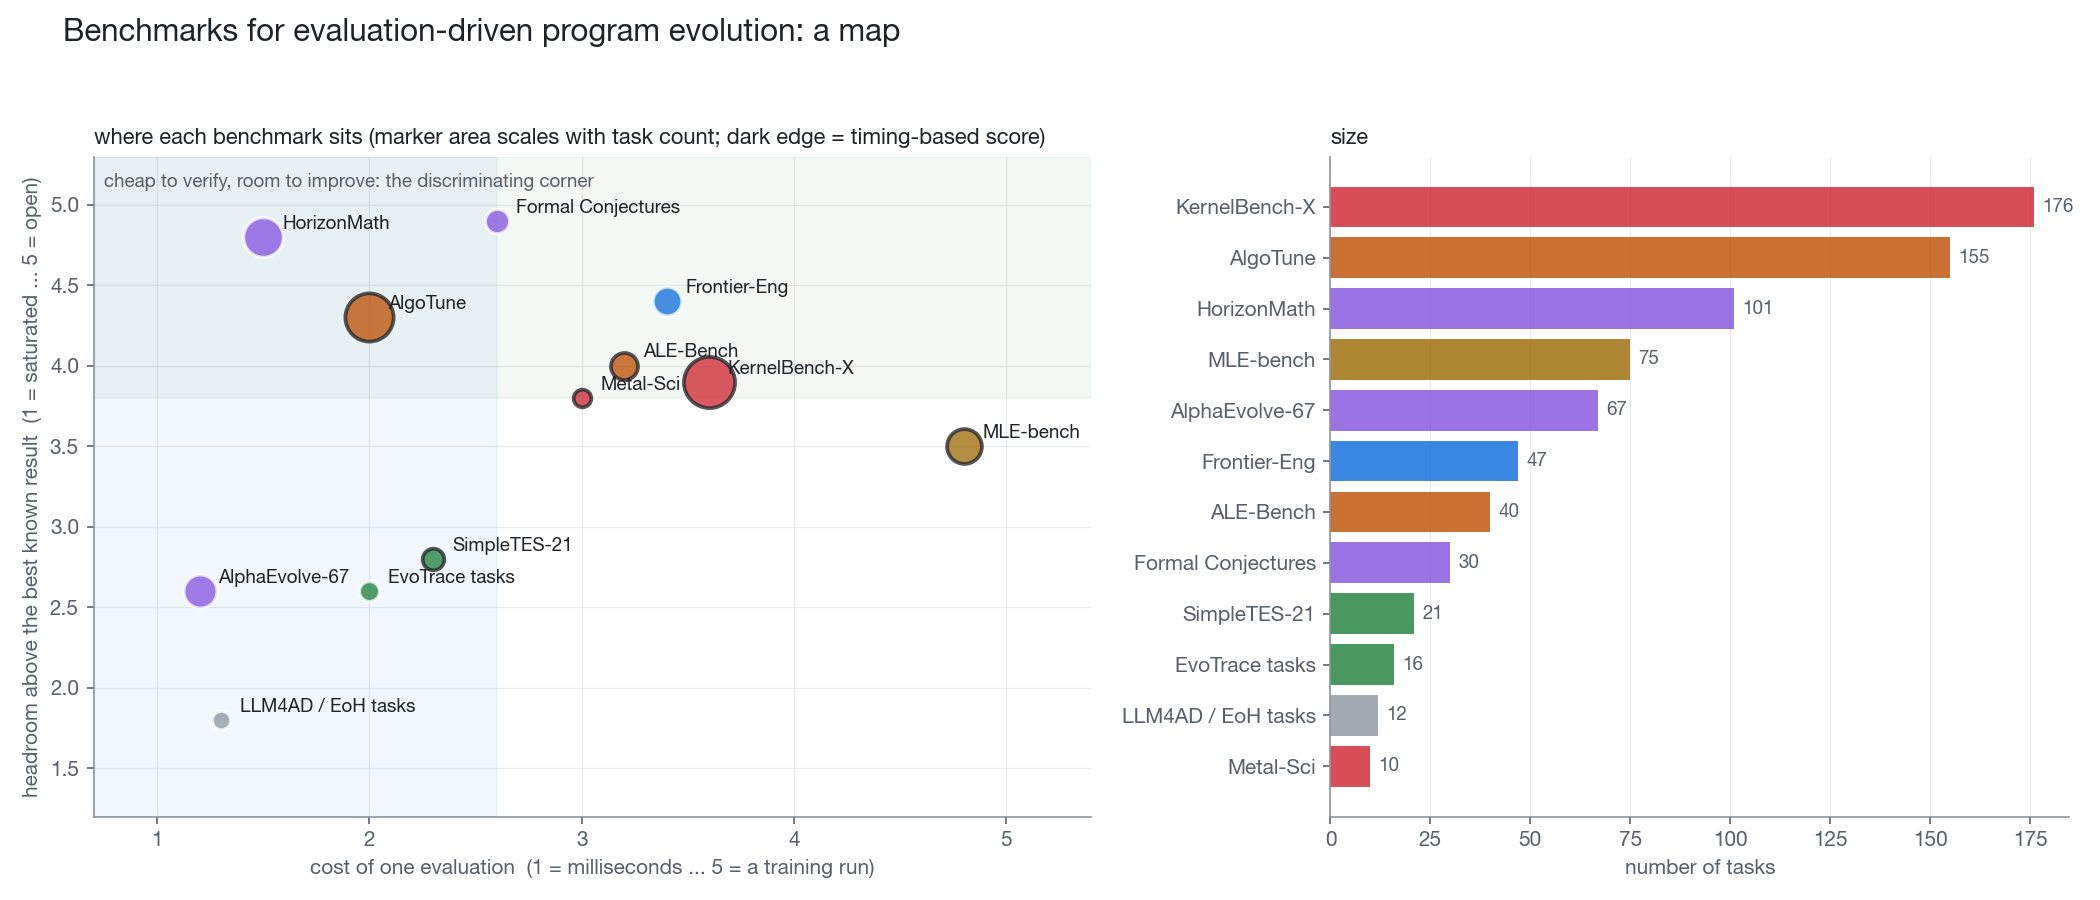
\includegraphics[width=\textwidth]{benchmarks_figs/overview_map.png}
\caption{The surveyed benchmarks placed by evaluation cost and headroom (both judged from the
papers, so qualitative), with task counts. The discriminating corner is cheap to verify and far
from saturation; AlgoTune, HorizonMath and Frontier-Eng sit in or near it.}
\end{figure}

\section{The benchmarks}

\subsection{AlphaEvolve's 67 problems (Tao, Georgiev, G\'omez-Serrano, Wagner, Nov 2025)}

The canonical set for this whole line of work. The paper applies AlphaEvolve --- an LLM
proposing program edits, an evaluator scoring them, an evolutionary loop keeping the best --- to
67 problems from mathematical analysis, combinatorics, geometry and number theory, each asking
for a construction that improves a known bound (packings, sum-vs-difference sets, autocorrelation
inequalities, kissing numbers, Kakeya and Nikodym sets, tilings, \ldots). The system rediscovered
the best known constructions in most cases, improved several, and in some cases generalized a
finite set of numerical results into a formula.

\facts{\textbf{67 problems} $\cdot$ 4 areas of mathematics $\cdot$ score: the bound achieved
$\cdot$ verification: exact, milliseconds to seconds $\cdot$ headroom: varies by problem; many now
matched by several systems $\cdot$ code: the problem statements and evaluators are in the paper's
companion notebooks. \href{https://arxiv.org/abs/2511.02864}{arXiv:2511.02864}}

\fit{Breadth is the value: 67 cheap, exact problems. The risk is the one we already met --- circle
packing and Erd\H{o}s are on this list and both saturate. Choose problems where the paper reports
an \emph{improvement} rather than a rediscovery; those still have a landscape.}

\subsection{HorizonMath (Mar 2026)}

Built explicitly for the ``discovery is hard, verification is cheap'' regime. 101 predominantly
\emph{unsolved} problems from eight areas of computational and applied mathematics (number
theory, lattice models, discrete geometry, continuum physics, combinatorics, integrals,
mathematical constants, coding theory), each with an automatic verifier in an open-source
framework. Because the answers are unknown the benchmark cannot be contaminated, and
state-of-the-art models score near 0\%. Problems are tiered by estimated solvability, from a
calibration tier to ``likely unsolvable''.

\begin{figure}[H]
\centering
\includegraphics[width=0.85\textwidth]{benchmarks_figs/horizonmath.png}
\caption{HorizonMath's composition: solvability tiers (left) and domains (right). Figure from
arXiv:2603.15617.}
\end{figure}

\facts{\textbf{101 problems} $\cdot$ 8 domains $\cdot$ score: verifier-defined, often a bound to
improve $\cdot$ verification: automatic, cheap by design $\cdot$ headroom: open --- these are
unsolved $\cdot$ code: \url{https://github.com/ewang26/HorizonMath}.
\href{https://arxiv.org/abs/2603.15617}{arXiv:2603.15617}}

\fit{The best match to criteria 1, 2 and 4 at once. A result here means something outside the
benchmark. The calibration and ``likely solvable'' tiers (33 problems) are where a search method
can show progress in a day's budget; the rest is for longer campaigns.}

\subsection{Formal Conjectures (May 2026)}

An evolving repository of 2\,615 problem statements formalized in Lean~4, of which 1\,029 are
open research conjectures and 836 are solved problems for autoformalization. Verification is a
Lean proof, so it is exact and contamination-free, and the repository has already been used to
resolve open conjectures.

\facts{1\,029 open conjectures $\cdot$ score: proved / not proved $\cdot$ verification: Lean
kernel $\cdot$ headroom: open. \href{https://arxiv.org/abs/2605.13171}{arXiv:2605.13171}}

\fit{Listed for completeness: it is a proof benchmark, binary, and outside the
construct-and-score paradigm our methods run in. Relevant only if we move to proof search.}

\subsection{SimpleTES's 21 problems (Apr 2026)}

The task set behind SimpleTES (``Structured Scaling of AI Discovery Across Diverse Scientific
Domains''): 21 open-ended problems across six domains --- mathematical constructions, scientific
algorithms, AI foundations (kernels, losses), quantum circuit compilation, astrodynamics
trajectory design, and more --- on which the authors report state-of-the-art results with an
open-weight model. Each task is a directory with an initial program, an evaluator and a
description: the same contract our bench uses, because we ported it.

\begin{figure}[H]
\centering
\includegraphics[width=0.9\textwidth]{benchmarks_figs/simpletes.png}
\caption{SimpleTES: the loop, the domains, and representative discoveries (qubit routing,
spacecraft trajectories, lasso solvers, a Triton kernel). Figure from arXiv:2604.19341.}
\end{figure}

\facts{\textbf{21 problems} $\cdot$ 6 domains $\cdot$ score: task-defined $\cdot$ verification:
per task; some are simulations (astrodynamics) or timed kernels $\cdot$ headroom: SimpleTES's own
numbers are the bar $\cdot$ code: \url{https://github.com/wq-will/SimpleTES}.
\href{https://arxiv.org/abs/2604.19341}{arXiv:2604.19341}}

\fit{Zero integration cost --- these run in \texttt{run\_bench.py} as they are --- and a
published baseline from the method our inner loop reproduces. Three of the 21 are our current
tasks; the other 18 are new to us.}

\subsection{ALE-Bench (Sakana AI, NeurIPS 2025)}

Score-based algorithm engineering from the AtCoder Heuristic Contests: 40 past problems
(package routing, crew scheduling, production planning, grid balancing) whose optima are out of
reach, with the official scorers and a sandbox that replicates the contest environment. Unlike
pass/fail coding benchmarks it is built for long-horizon refinement with test-run feedback, and
it reports where AI systems stand relative to human contestants. A 10-problem ``lite'' subset
exists. Our AHC039 is one of its problems.

\facts{\textbf{40 problems} (lite: 10) $\cdot$ score: contest score, per case $\cdot$
verification: official scorer; \emph{wall-clock limited}, so noisy $\cdot$ headroom: real ---
top humans are far ahead $\cdot$ code: \url{https://github.com/SakanaAI/ALE-Bench}.
\href{https://arxiv.org/abs/2506.09050}{arXiv:2506.09050}}

\fit{The natural continuation of the AHC039 line, and the only suite here where our LabNotebook
result (3749--3769 against seeds near 3700) has headroom above it. Requires the dedicated
evaluation server we already built; budget one machine per wave.}

\subsection{AlgoTune (NeurIPS 2025)}

154 numerical tasks from computer science, physics and mathematics (QR decomposition, gzip,
PageRank, convex programs, graph algorithms, \ldots), each with a reference implementation from a
standard package (SciPy, scikit-learn, CVXPY, NetworkX). The score is the \textbf{speedup} of the
candidate over the reference on validated outputs, so it is continuous and unbounded. The
baseline agent, AlgoTuner, reaches a mean $1.72\times$; the authors' finding is that current
models mostly make surface-level optimizations rather than algorithmic ones.

\begin{figure}[H]
\centering
\includegraphics[width=0.85\textwidth]{benchmarks_figs/algotune.png}
\caption{AlgoTune's protocol: pick a task, optimize the code, time it against the reference.
Figure from arXiv:2507.15887.}
\end{figure}

\facts{\textbf{154 tasks} $\cdot$ score: speedup ratio, correctness checked separately $\cdot$
verification: exact correctness; timing has noise but is controllable (fixed inputs, repeats)
$\cdot$ headroom: unbounded by construction $\cdot$ code: \url{https://github.com/oripress/AlgoTune}.
\href{https://arxiv.org/abs/2507.15887}{arXiv:2507.15887}}

\fit{No ceiling, exact correctness, hundreds of cheap evaluations per arm. The ``surface vs.\
algorithmic change'' question the authors raise is exactly what a notebook-style search should be
judged on, and EvoTrace-style attribution can answer it from our digests.}

\subsection{Frontier-Eng (Apr 2026)}

A human-verified benchmark for \emph{generative optimization}: an agent proposes an artifact
(a control waveform, a circuit layout, a truss, a schedule, a quantum circuit), an
industrial-grade simulator scores it with a continuous reward under hard feasibility
constraints, and the agent revises within a fixed interaction budget. 47 tasks in five domains:
computing and quantum information, operations research and decision science, robotics and
control, optics and communication systems, physical sciences and engineering design. Eight
frontier models are benchmarked under representative search frameworks, with anti-hack
safeguards (read-only evaluators, sandboxed execution).

\begin{figure}[H]
\centering
\includegraphics[width=0.8\textwidth]{benchmarks_figs/frontiereng.png}
\caption{Frontier-Eng: why pass/fail benchmarks miss iterative optimization, and the
propose--evaluate--revise loop with its safeguards. Figure from arXiv:2604.12290.}
\end{figure}

\facts{\textbf{47 tasks} $\cdot$ 5 engineering domains $\cdot$ score: continuous reward with
hard constraints $\cdot$ verification: simulators, seconds to minutes $\cdot$ headroom: real;
frontier models are far from the human-verified references $\cdot$
\href{https://arxiv.org/abs/2604.12290}{arXiv:2604.12290}}

\fit{Designed for exactly our protocol --- a budgeted propose--execute--evaluate loop --- with
continuous rewards and constraints. Evaluations are heavier than a packing check but still cheap
against a model call. One task per domain gives five very different landscapes.}

\subsection{KernelBench, KernelBench-X, and Metal-Sci (2025--2026)}

GPU kernel generation. \textbf{KernelBench} (Feb 2025) has 250 PyTorch workloads and the
\texttt{fast\_p} metric: the fraction of generated kernels that are correct \emph{and} faster
than the baseline by a threshold. \textbf{KernelBench-X} (May 2026) re-organizes the space into
176 Triton tasks in 15 categories and finds that task category explains far more of the
correctness variance than the method does (72\% of fusion tasks fail under every method), and that
iterative refinement raises compile rates without raising speedups. \textbf{Metal-Sci} (May 2026)
is a 10-task benchmark of scientific Metal compute kernels (stencils, $n$-body, Boltzmann,
molecular dynamics, PDEs, FFT) for \emph{evolutionary} LLM search on Apple Silicon, with a
roofline-anchored fitness and a held-out size to catch overfitting; on an M1 Pro it reports
self-speedups from $1.0\times$ to $10.7\times$.

\begin{figure}[H]
\centering
\includegraphics[width=0.72\textwidth]{benchmarks_figs/kernelbenchx.png}
\caption{KernelBench-X's shared evaluation pipeline for candidate kernels. Figure from
arXiv:2605.04956.}
\end{figure}

\facts{KernelBench 250 / KernelBench-X 176 / Metal-Sci 10 tasks $\cdot$ score: correctness +
speedup $\cdot$ verification: run on hardware; timing noise $\cdot$ headroom: large $\cdot$
hardware: CUDA GPUs, or an M-series Mac for Metal-Sci.
\href{https://arxiv.org/abs/2502.10517}{arXiv:2502.10517},
\href{https://arxiv.org/html/2605.04956v1}{arXiv:2605.04956},
\href{https://arxiv.org/pdf/2605.09708}{arXiv:2605.09708}}

\fit{Strong headroom, but timing-based scores and hardware requirements. Metal-Sci is the one
that runs locally on the machine we already have; it is also built for a $(1{+}1)$ evolutionary
loop, so our operators drop in.}

\subsection{Heuristic design: LLM4AD, EoH, ReEvo, FunSearch tasks (2023--2025)}

The lineage that began with FunSearch (cap sets, online bin packing) and continued with EoH and
ReEvo: evolve a \emph{heuristic function} for a combinatorial problem --- TSP, CVRP, online bin
packing, knapsack, job-shop scheduling --- scored by the objective gap against a strong baseline
heuristic on standard instances. \textbf{LLM4AD} packages these tasks, several search methods
and a sandboxed evaluator in one platform, spanning optimization, machine learning and science
tasks.

\begin{figure}[H]
\centering
\includegraphics[width=0.7\textwidth]{benchmarks_figs/llm4ad.png}
\caption{LLM4AD: models, task families and search methods behind one interface. Figure from
arXiv:2412.17287.}
\end{figure}

\facts{$\sim$12 standard tasks (more in LLM4AD) $\cdot$ score: objective gap to a baseline
heuristic $\cdot$ verification: exact, cheap $\cdot$ headroom: limited --- the good heuristics are
well known to models $\cdot$ code: \url{https://github.com/Optima-CityU/LLM4AD}.
\href{https://arxiv.org/abs/2412.17287}{arXiv:2412.17287}}

\fit{Cheap and standard, with published baselines for EoH and ReEvo --- the two closest
relatives of LabNotebook --- which makes it the right place for a head-to-head against them. Expect
saturation within a run; the comparison is about the path, not the endpoint.}

\subsection{MLE-bench (OpenAI, Oct 2024)}

75 Kaggle competitions (tabular, vision, NLP), scored against the public leaderboards as medal
rates and percentiles, with human baselines. The AIDE scaffold with o1-preview reached a bronze
medal or better in 16.9\% of competitions; the paper studies resource scaling and contamination.

\facts{\textbf{75 competitions} $\cdot$ score: leaderboard percentile / medal $\cdot$
verification: held-out test set, exact $\cdot$ cost: each evaluation is a training run ---
minutes to hours $\cdot$ code: \url{https://github.com/openai/mle-bench}.
\href{https://arxiv.org/abs/2410.07095}{arXiv:2410.07095}}

\fit{The search-over-scripts arena (AIDE, MLE-STAR). Our methods fit, but evaluation cost means a
budget buys tens of candidates, not hundreds; and the ``time limit'' effects we saw on Erd\H{o}s
would dominate. Not a first choice.}

\subsection{EvoTrace (May 2026) --- a task set for attribution}

Not a benchmark of scores but of \emph{traces}: runs of four evolutionary frameworks with
reasoning and non-reasoning models on 16 tasks in mathematics and algorithm design, annotated so
that each improving edit can be attributed to new algorithmic structure, re-tuning, recombination
of known ideas, or evaluator overfitting. The paper's point is that the final score alone cannot
tell these apart.

\begin{figure}[H]
\centering
\includegraphics[width=0.8\textwidth]{benchmarks_figs/evotrace.png}
\caption{EvoTrace's taxonomy of edits, from bug fixes and hyper-parameter changes to
architectural change. Figure from arXiv:2605.20086.}
\end{figure}

\facts{\textbf{16 tasks} $\cdot$ 4 frameworks $\cdot$ score: their originals, plus edit-type
labels $\cdot$ \href{https://arxiv.org/abs/2605.20086}{arXiv:2605.20086}}

\fit{Adopting its 16 tasks buys comparability with four published frameworks, and its edit
taxonomy is the analysis LabNotebook's digests already produce in prose --- a chance to validate
the notebook's attributions against an independent labeling.}

\section{Side by side}

\begin{center}\small
\begin{tabular}{@{}>{\raggedright\arraybackslash}p{30mm}rp{24mm}p{22mm}p{18mm}p{44mm}@{}}
\toprule
benchmark & tasks & score & verification & headroom & fit \\
\midrule
AlphaEvolve-67 & 67 & bound & exact, ms & mixed & breadth; avoid the saturated ones \\
HorizonMath & 101 & bound / verifier & exact, cheap & open & best discovery signal \\
Formal Conjectures & 1\,029 & proved? & Lean & open & proof search only \\
SimpleTES-21 & 21 & task-defined & mixed & moderate & runs today; baseline exists \\
ALE-Bench & 40 & contest score & wall-clock & real & AHC039 continuation; needs eval server \\
AlgoTune & 154 & speedup & exact + timing & unbounded & no ceiling; cheap \\
Frontier-Eng & 47 & continuous reward & simulators & real & built for budgeted loops \\
KernelBench-X & 176 & correct + speedup & GPU timing & large & needs GPUs \\
Metal-Sci & 10 & roofline speedup & Metal timing & large & runs on our Mac \\
LLM4AD / EoH tasks & $\sim$12 & objective gap & exact, cheap & limited & EoH/ReEvo head-to-head \\
MLE-bench & 75 & leaderboard & training runs & moderate & too expensive per eval \\
EvoTrace tasks & 16 & originals & exact & mixed & comparability + attribution \\
\bottomrule
\end{tabular}
\end{center}

\section{Recommendation}

For ranking search methods --- the purpose our current three tasks could not serve --- the next
suite should be drawn from the discriminating corner of Figure~1:

\begin{enumerate}
  \item \textbf{AlgoTune, a 10-task subset.} Exact correctness, unbounded speedup, evaluations in
    seconds. Four methods $\times$ three seeds is one afternoon of compute, and it tests directly
    whether a method produces algorithmic change or tuning --- the distinction our AHC039 digests
    already make in prose.
  \item \textbf{Frontier-Eng, one task per domain.} Continuous reward under hard constraints, a
    fixed budget, five unrelated landscapes.
  \item \textbf{HorizonMath, the calibration and likely-solvable tiers.} For the discovery claim:
    no ceiling, no contamination, a verifier that costs nothing.
\end{enumerate}

\noindent Alongside: \textbf{ALE-Bench lite} to continue the AHC039 line on the serialized
evaluation server, and \textbf{SimpleTES-21} as the zero-integration option with a published
baseline. Defer the kernel benchmarks unless we spend on GPUs --- except Metal-Sci, which runs on
the machine at hand. In every case the seed-quality control from the MERFISH panel study applies:
a benchmark where the seed already sits at the ceiling measures nothing about the search.

\vfill
\noindent\footnotesize Figures reproduced from the cited papers (arXiv HTML renderings), for
internal reference.\\
Fetched by \texttt{fetch\_benchmark\_figs.py}; placement in Figure~1 is a judgment from the papers,
not a measurement.
\end{document}
